% ============================================================
% state_diagram.tex
% Máquina de estados UML — Ciclo de vida del Pedido (P3)
% ISR-401 — Prueba Práctica Unidad IV
% ============================================================
% Este archivo puede compilarse de forma independiente o
% incluirse desde main.tex con % ============================================================
% state_diagram.tex
% Máquina de estados UML — Ciclo de vida del Pedido (P3)
% ISR-401 — Prueba Práctica Unidad IV
% ============================================================
% Este archivo puede compilarse de forma independiente o
% incluirse desde main.tex con % ============================================================
% state_diagram.tex
% Máquina de estados UML — Ciclo de vida del Pedido (P3)
% ISR-401 — Prueba Práctica Unidad IV
% ============================================================
% Este archivo puede compilarse de forma independiente o
% incluirse desde main.tex con % ============================================================
% state_diagram.tex
% Máquina de estados UML — Ciclo de vida del Pedido (P3)
% ISR-401 — Prueba Práctica Unidad IV
% ============================================================
% Este archivo puede compilarse de forma independiente o
% incluirse desde main.tex con \input{diagramas/state_diagram}
% ============================================================

\documentclass[tikz,border=10pt]{standalone}
\usepackage{tikz}
\usetikzlibrary{shapes.geometric, positioning, arrows.meta, fit, backgrounds}

\begin{document}
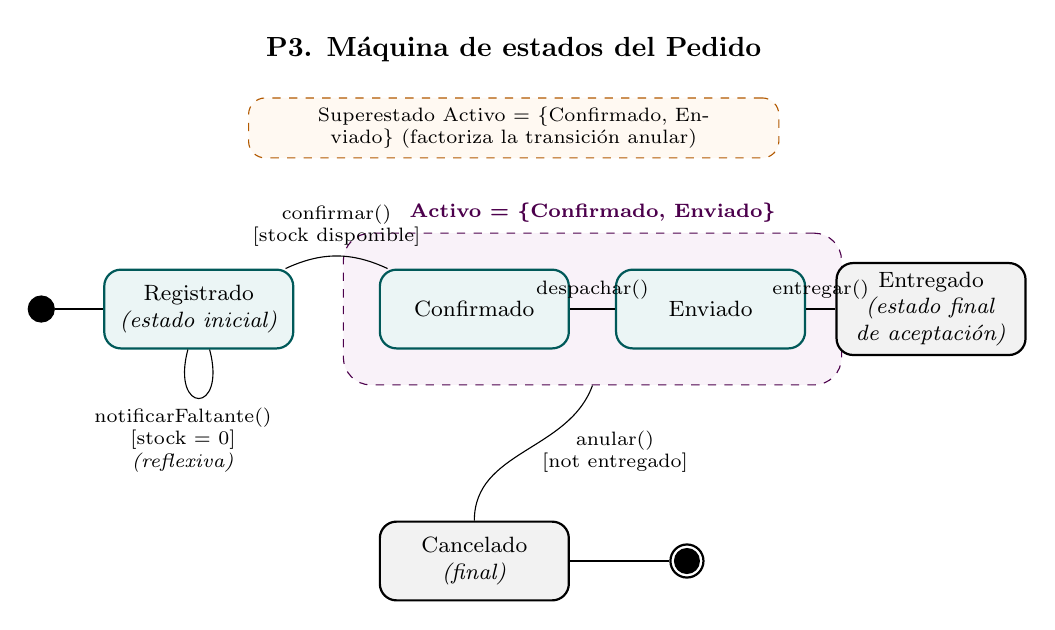
\begin{tikzpicture}[
    state/.style={rectangle, rounded corners=6pt, draw=teal!70!black, thick,
        fill=teal!8, minimum width=2.4cm, minimum height=1cm, align=center, font=\footnotesize},
    finalstate/.style={rectangle, rounded corners=6pt, draw=black, thick,
        fill=gray!10, minimum width=2.4cm, minimum height=1cm, align=center, font=\footnotesize},
    initial/.style={circle, draw=black, fill=black, minimum size=0.3cm},
    finaldot/.style={circle, draw=black, thick, fill=white, minimum size=0.42cm},
    finaldotinner/.style={circle, fill=black, minimum size=0.18cm},
    every edge/.style={draw, -{Stealth[length=2.5mm]}, thick},
    lbl/.style={font=\scriptsize, align=center}
]

% --- Título ---
\node[font=\bfseries] at (6,7.3) {P3. Máquina de estados del Pedido};

% --- Estados principales ---
\node[initial] (ini) at (0,4) {};
\node[state] (registrado) at (2,4) {Registrado\\\textit{(estado inicial)}};
\node[state] (confirmado) at (5.5,4) {Confirmado};
\node[state] (enviado) at (8.5,4) {Enviado};
\node[finalstate] (entregado) at (11.3,4) {Entregado\\\textit{(estado final}\\\textit{de aceptación)}};

\node[finalstate] (cancelado) at (5.5,0.8) {Cancelado\\\textit{(final)}};
\node[finaldot] (finC) at (8.2,0.8) {};
\node[finaldotinner] at (finC) {};

% --- Superestado Activo ---
\begin{scope}[on background layer]
\node[draw=violet!60!black, dashed, rounded corners=10pt, fill=violet!5,
    fit=(confirmado)(enviado), inner sep=0.45cm, label={[font=\scriptsize\bfseries, violet!60!black]above:Activo = \{Confirmado, Enviado\}}] (activo) {};
\end{scope}

\node[draw=orange!70!black, dashed, rounded corners=6pt, fill=orange!5,
    text width=6.5cm, align=center, font=\scriptsize] at (6,6.3)
    {Superestado Activo = \{Confirmado, Enviado\} (factoriza la transición anular)};

% --- Transiciones ---
\draw (ini) -- (registrado);

\draw (registrado) to[bend left=25] node[lbl, above] {confirmar()\\{[stock disponible]}} (confirmado);

\draw (registrado) to[loop below, looseness=8] node[lbl, below, xshift=-0.2cm]
    {notificarFaltante()\\{[stock = 0]}\\\textit{(reflexiva)}} (registrado);


\draw (confirmado) -- node[lbl, above] {despachar()} (enviado);
\draw (enviado) -- node[lbl, above] {entregar()} (entregado);

% --- Transición factorizada anular() desde el superestado Activo ---
\draw (activo.south) to[out=250,in=90] node[lbl, right, xshift=0.1cm]
    {anular()\\{[not entregado]}} (cancelado.north);

\draw (cancelado) -- (finC);

\end{tikzpicture}
\end{document}

% ============================================================

\documentclass[tikz,border=10pt]{standalone}
\usepackage{tikz}
\usetikzlibrary{shapes.geometric, positioning, arrows.meta, fit, backgrounds}

\begin{document}
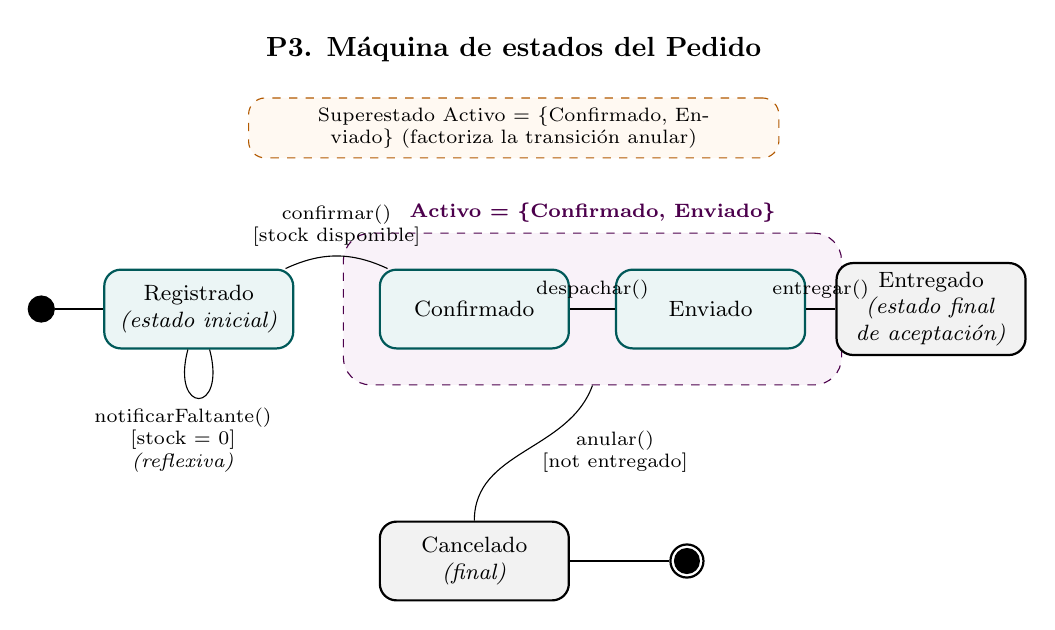
\begin{tikzpicture}[
    state/.style={rectangle, rounded corners=6pt, draw=teal!70!black, thick,
        fill=teal!8, minimum width=2.4cm, minimum height=1cm, align=center, font=\footnotesize},
    finalstate/.style={rectangle, rounded corners=6pt, draw=black, thick,
        fill=gray!10, minimum width=2.4cm, minimum height=1cm, align=center, font=\footnotesize},
    initial/.style={circle, draw=black, fill=black, minimum size=0.3cm},
    finaldot/.style={circle, draw=black, thick, fill=white, minimum size=0.42cm},
    finaldotinner/.style={circle, fill=black, minimum size=0.18cm},
    every edge/.style={draw, -{Stealth[length=2.5mm]}, thick},
    lbl/.style={font=\scriptsize, align=center}
]

% --- Título ---
\node[font=\bfseries] at (6,7.3) {P3. Máquina de estados del Pedido};

% --- Estados principales ---
\node[initial] (ini) at (0,4) {};
\node[state] (registrado) at (2,4) {Registrado\\\textit{(estado inicial)}};
\node[state] (confirmado) at (5.5,4) {Confirmado};
\node[state] (enviado) at (8.5,4) {Enviado};
\node[finalstate] (entregado) at (11.3,4) {Entregado\\\textit{(estado final}\\\textit{de aceptación)}};

\node[finalstate] (cancelado) at (5.5,0.8) {Cancelado\\\textit{(final)}};
\node[finaldot] (finC) at (8.2,0.8) {};
\node[finaldotinner] at (finC) {};

% --- Superestado Activo ---
\begin{scope}[on background layer]
\node[draw=violet!60!black, dashed, rounded corners=10pt, fill=violet!5,
    fit=(confirmado)(enviado), inner sep=0.45cm, label={[font=\scriptsize\bfseries, violet!60!black]above:Activo = \{Confirmado, Enviado\}}] (activo) {};
\end{scope}

\node[draw=orange!70!black, dashed, rounded corners=6pt, fill=orange!5,
    text width=6.5cm, align=center, font=\scriptsize] at (6,6.3)
    {Superestado Activo = \{Confirmado, Enviado\} (factoriza la transición anular)};

% --- Transiciones ---
\draw (ini) -- (registrado);

\draw (registrado) to[bend left=25] node[lbl, above] {confirmar()\\{[stock disponible]}} (confirmado);

\draw (registrado) to[loop below, looseness=8] node[lbl, below, xshift=-0.2cm]
    {notificarFaltante()\\{[stock = 0]}\\\textit{(reflexiva)}} (registrado);


\draw (confirmado) -- node[lbl, above] {despachar()} (enviado);
\draw (enviado) -- node[lbl, above] {entregar()} (entregado);

% --- Transición factorizada anular() desde el superestado Activo ---
\draw (activo.south) to[out=250,in=90] node[lbl, right, xshift=0.1cm]
    {anular()\\{[not entregado]}} (cancelado.north);

\draw (cancelado) -- (finC);

\end{tikzpicture}
\end{document}

% ============================================================

\documentclass[tikz,border=10pt]{standalone}
\usepackage{tikz}
\usetikzlibrary{shapes.geometric, positioning, arrows.meta, fit, backgrounds}

\begin{document}
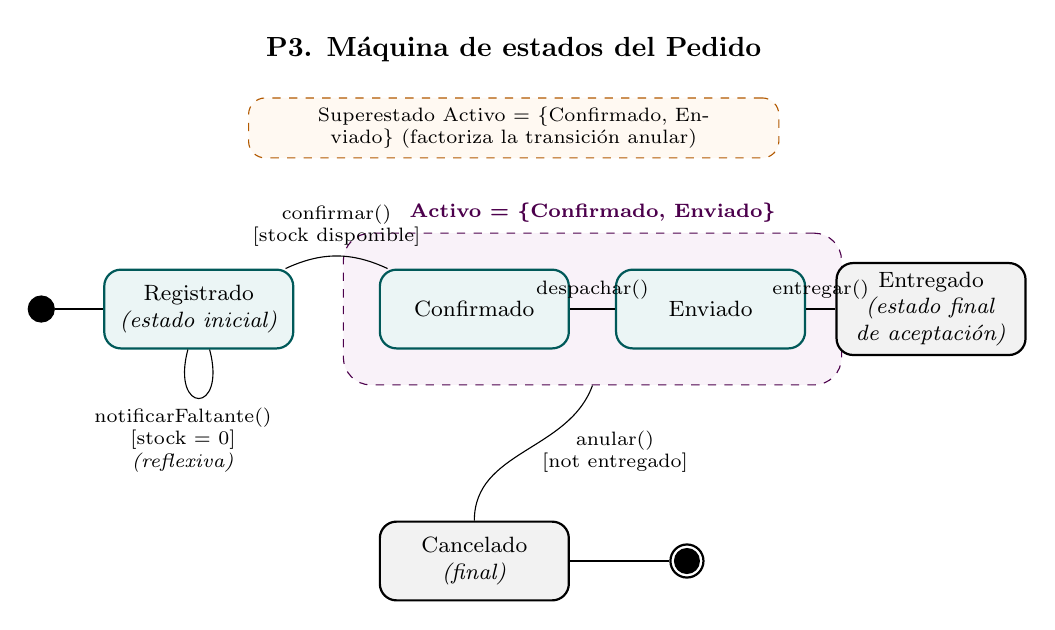
\begin{tikzpicture}[
    state/.style={rectangle, rounded corners=6pt, draw=teal!70!black, thick,
        fill=teal!8, minimum width=2.4cm, minimum height=1cm, align=center, font=\footnotesize},
    finalstate/.style={rectangle, rounded corners=6pt, draw=black, thick,
        fill=gray!10, minimum width=2.4cm, minimum height=1cm, align=center, font=\footnotesize},
    initial/.style={circle, draw=black, fill=black, minimum size=0.3cm},
    finaldot/.style={circle, draw=black, thick, fill=white, minimum size=0.42cm},
    finaldotinner/.style={circle, fill=black, minimum size=0.18cm},
    every edge/.style={draw, -{Stealth[length=2.5mm]}, thick},
    lbl/.style={font=\scriptsize, align=center}
]

% --- Título ---
\node[font=\bfseries] at (6,7.3) {P3. Máquina de estados del Pedido};

% --- Estados principales ---
\node[initial] (ini) at (0,4) {};
\node[state] (registrado) at (2,4) {Registrado\\\textit{(estado inicial)}};
\node[state] (confirmado) at (5.5,4) {Confirmado};
\node[state] (enviado) at (8.5,4) {Enviado};
\node[finalstate] (entregado) at (11.3,4) {Entregado\\\textit{(estado final}\\\textit{de aceptación)}};

\node[finalstate] (cancelado) at (5.5,0.8) {Cancelado\\\textit{(final)}};
\node[finaldot] (finC) at (8.2,0.8) {};
\node[finaldotinner] at (finC) {};

% --- Superestado Activo ---
\begin{scope}[on background layer]
\node[draw=violet!60!black, dashed, rounded corners=10pt, fill=violet!5,
    fit=(confirmado)(enviado), inner sep=0.45cm, label={[font=\scriptsize\bfseries, violet!60!black]above:Activo = \{Confirmado, Enviado\}}] (activo) {};
\end{scope}

\node[draw=orange!70!black, dashed, rounded corners=6pt, fill=orange!5,
    text width=6.5cm, align=center, font=\scriptsize] at (6,6.3)
    {Superestado Activo = \{Confirmado, Enviado\} (factoriza la transición anular)};

% --- Transiciones ---
\draw (ini) -- (registrado);

\draw (registrado) to[bend left=25] node[lbl, above] {confirmar()\\{[stock disponible]}} (confirmado);

\draw (registrado) to[loop below, looseness=8] node[lbl, below, xshift=-0.2cm]
    {notificarFaltante()\\{[stock = 0]}\\\textit{(reflexiva)}} (registrado);


\draw (confirmado) -- node[lbl, above] {despachar()} (enviado);
\draw (enviado) -- node[lbl, above] {entregar()} (entregado);

% --- Transición factorizada anular() desde el superestado Activo ---
\draw (activo.south) to[out=250,in=90] node[lbl, right, xshift=0.1cm]
    {anular()\\{[not entregado]}} (cancelado.north);

\draw (cancelado) -- (finC);

\end{tikzpicture}
\end{document}

% ============================================================

\documentclass[tikz,border=10pt]{standalone}
\usepackage{tikz}
\usetikzlibrary{shapes.geometric, positioning, arrows.meta, fit, backgrounds}

\begin{document}
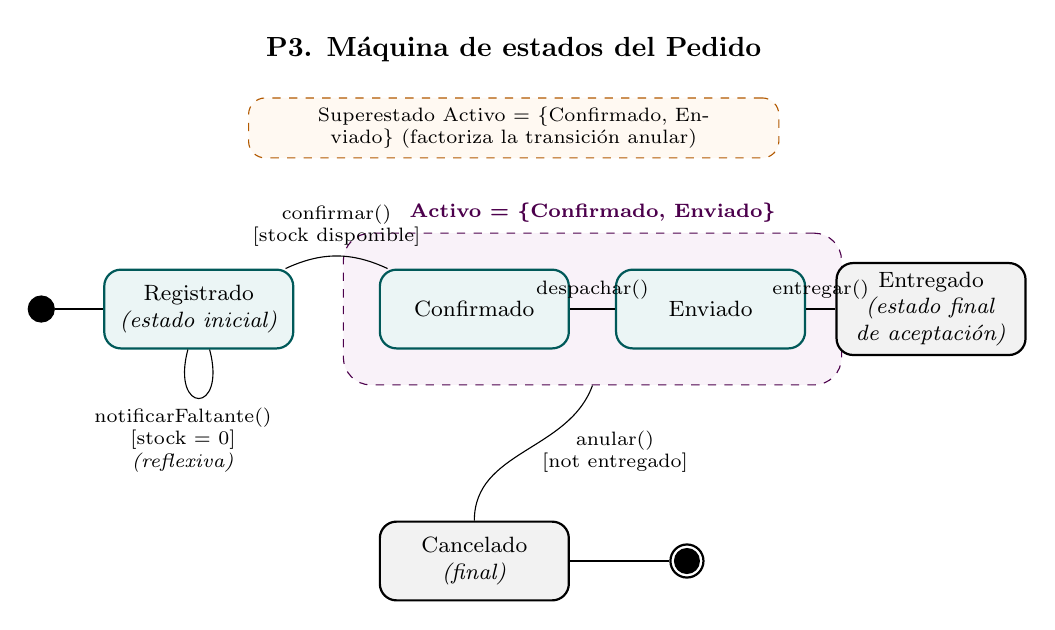
\begin{tikzpicture}[
    state/.style={rectangle, rounded corners=6pt, draw=teal!70!black, thick,
        fill=teal!8, minimum width=2.4cm, minimum height=1cm, align=center, font=\footnotesize},
    finalstate/.style={rectangle, rounded corners=6pt, draw=black, thick,
        fill=gray!10, minimum width=2.4cm, minimum height=1cm, align=center, font=\footnotesize},
    initial/.style={circle, draw=black, fill=black, minimum size=0.3cm},
    finaldot/.style={circle, draw=black, thick, fill=white, minimum size=0.42cm},
    finaldotinner/.style={circle, fill=black, minimum size=0.18cm},
    every edge/.style={draw, -{Stealth[length=2.5mm]}, thick},
    lbl/.style={font=\scriptsize, align=center}
]

% --- Título ---
\node[font=\bfseries] at (6,7.3) {P3. Máquina de estados del Pedido};

% --- Estados principales ---
\node[initial] (ini) at (0,4) {};
\node[state] (registrado) at (2,4) {Registrado\\\textit{(estado inicial)}};
\node[state] (confirmado) at (5.5,4) {Confirmado};
\node[state] (enviado) at (8.5,4) {Enviado};
\node[finalstate] (entregado) at (11.3,4) {Entregado\\\textit{(estado final}\\\textit{de aceptación)}};

\node[finalstate] (cancelado) at (5.5,0.8) {Cancelado\\\textit{(final)}};
\node[finaldot] (finC) at (8.2,0.8) {};
\node[finaldotinner] at (finC) {};

% --- Superestado Activo ---
\begin{scope}[on background layer]
\node[draw=violet!60!black, dashed, rounded corners=10pt, fill=violet!5,
    fit=(confirmado)(enviado), inner sep=0.45cm, label={[font=\scriptsize\bfseries, violet!60!black]above:Activo = \{Confirmado, Enviado\}}] (activo) {};
\end{scope}

\node[draw=orange!70!black, dashed, rounded corners=6pt, fill=orange!5,
    text width=6.5cm, align=center, font=\scriptsize] at (6,6.3)
    {Superestado Activo = \{Confirmado, Enviado\} (factoriza la transición anular)};

% --- Transiciones ---
\draw (ini) -- (registrado);

\draw (registrado) to[bend left=25] node[lbl, above] {confirmar()\\{[stock disponible]}} (confirmado);

\draw (registrado) to[loop below, looseness=8] node[lbl, below, xshift=-0.2cm]
    {notificarFaltante()\\{[stock = 0]}\\\textit{(reflexiva)}} (registrado);


\draw (confirmado) -- node[lbl, above] {despachar()} (enviado);
\draw (enviado) -- node[lbl, above] {entregar()} (entregado);

% --- Transición factorizada anular() desde el superestado Activo ---
\draw (activo.south) to[out=250,in=90] node[lbl, right, xshift=0.1cm]
    {anular()\\{[not entregado]}} (cancelado.north);

\draw (cancelado) -- (finC);

\end{tikzpicture}
\end{document}
